\documentclass{standalone}
\usepackage{tikz}
\usetikzlibrary{decorations.pathreplacing, calligraphy}

\tikzset{
  svgfrag/.style 2 args={
    execute at begin scope={\special{dvisvgm:raw <g class="fragment #2" data-fragment-index="#1">}},
    execute at end scope={\special{dvisvgm:raw </g>}},
    execute at begin node={\special{dvisvgm:raw <g class="fragment #2" data-fragment-index="#1">}},
    execute at end node={\special{dvisvgm:raw </g>}},
  }
}

\begin{document}
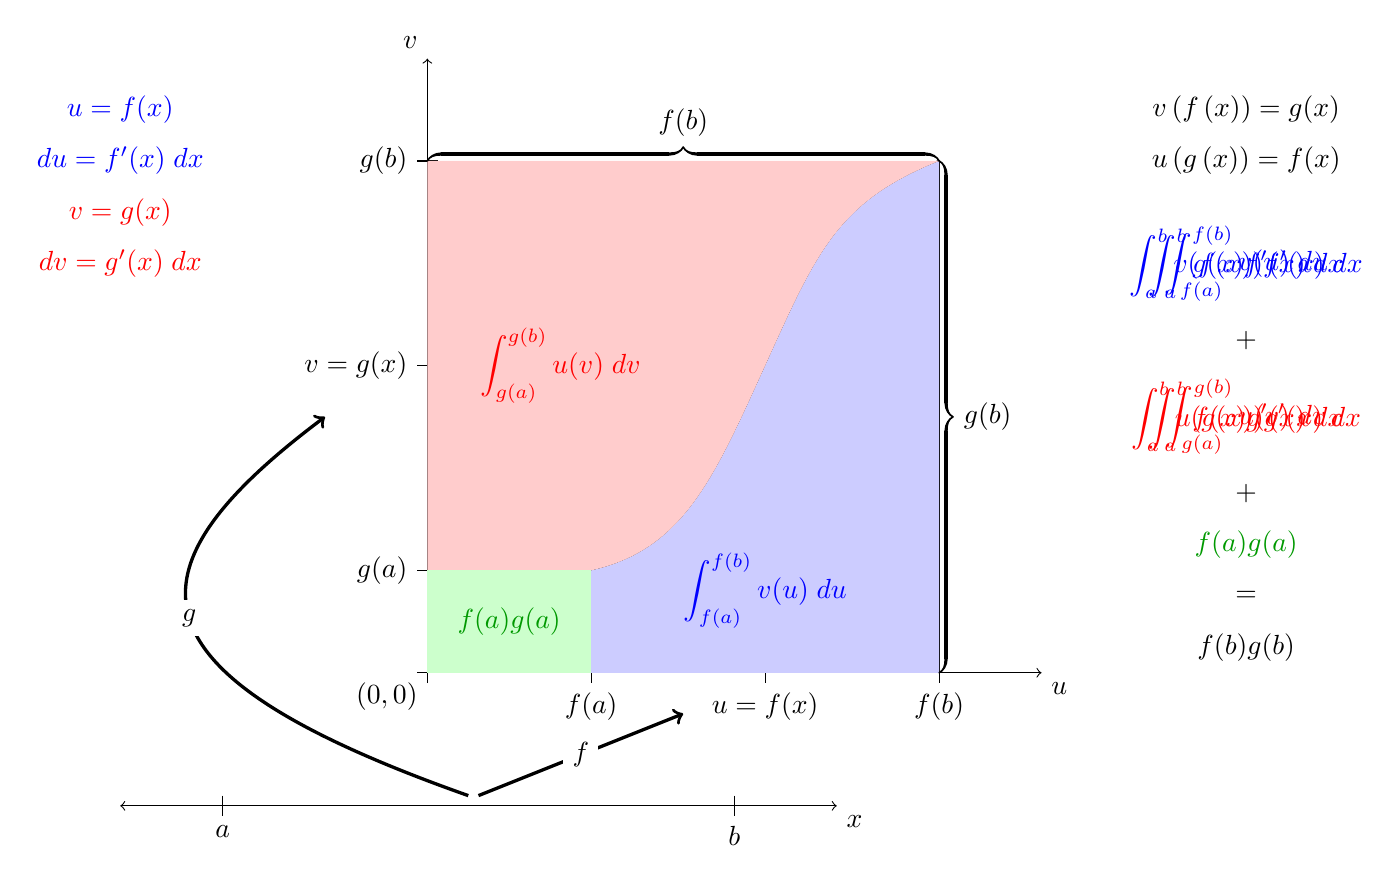
\begin{tikzpicture}[scale=1.3]
    \draw[thin, ->] (-.1,0) -- (6,0)node[below right]{$u$};
    \draw[thin, ->] (0, -.1) -- (0, 6)node[above left]{$v$};
    \draw[thin, <->] (-3,-1.3) -- (4,-1.3)node[below right]{$x$};
    \draw[thin] (-2,-1.3) +(0,.1) -- +(0,-.1)node[below]{$a$};
    \draw[thin] (3,-1.3) +(0,.1) -- +(0,-.1)node[below]{$b$};
    \node[below left] at (0,0) {$(0,0)$};
    \begin{scope}[svgfrag={1}{fade-in}]
        \draw[very thick,->] (0.5, -1.2) --node[fill=white]{$f$} (2.5, -.4);
        \draw[thin] (1.6,0) +(0,.1) --+(0,-.1)node[below]{$f(a)$};
        \draw[thin] (5,0) +(0,.1) --+(0,-.1)node[below]{$f(b)$};
        \draw[thin] (3.3,0) +(0,.1) --+(0,-.1)node[below]{$u = f(x)$};
    \end{scope}
    \begin{scope}[svgfrag={2}{fade-in}]
        \draw[very thick,->] (0.4, -1.2) ..controls(-3,0)and(-3,1)
        ..node[fill=white]{$g$} (-1, 2.5);
        \draw[thin] (0, 1) +(.1, 0) --+(-.1, 0)node[left]{$g(a)$};
        \draw[thin] (0, 5) +(.1, 0) --+(-.1, 0)node[left]{$g(b)$};
        \draw[thin] (0, 3) +(.1, 0) --+(-.1, 0)node[left]{$v = g(x)$};
    \end{scope}
    \begin{scope}[svgfrag={3}{fade-in}]
        \draw[thick] (1.6, 1) ..controls+(.9,.2) and +(-.5,-1.1) .. (3.3,3)
        ..controls+(.5,1.1) and +(-1,-.4) .. (5,5);
        \draw[very thin] (1.6,0) -- (1.6,1) -- (0,1);
        \draw[very thin] (5,0) -- (5,5) -- (0,5);
        \draw[thin, dashed] (3.3,0) -- (3.3,3)node[right]{$\left(f(x),g(x)\right)$} -- (0,3);
        \node at (8,5.5) {$\displaystyle v\left(f\left(x\right)\right) = g(x)$};
        \node at (8,5) {$\displaystyle u\left(g\left(x\right)\right) = f(x)$};
    \end{scope}
    \begin{scope}[svgfrag={4}{fade-in}]
        \fill[blue!20] (1.6,0) -- (1.6, 1) ..controls+(.9,.2) and +(-.5,-1.1) .. (3.3,3)
        ..controls+(.5,1.1) and +(-1,-.4) .. (5,5) -- (5,0) -- cycle;
        \node[blue] at (3.3,0.8){$\displaystyle \int_{f(a)}^{f(b)} v(u)\;du$};
        \node[blue, svgfrag={9}{fade-out}] at (8,4) {$\displaystyle \int_{f(a)}^{f(b)} v(u)\;du$};
    \end{scope}
    \begin{scope}[svgfrag={5}{fade-in}]
        \fill[red!20] (0,1) -- (1.6, 1) ..controls+(.9,.2) and +(-.5,-1.1) .. (3.3,3)
        ..controls+(.5,1.1) and +(-1,-.4) .. (5,5) -- (0,5) -- cycle;
        \node[red] at (1.3,3){$\displaystyle \int_{g(a)}^{g(b)} u(v)\;dv$};
        \node[red, svgfrag={11}{fade-out}] at (8,2.5) {$\displaystyle \int_{g(a)}^{g(b)} u(v)\;dv$};
        \node[black] at (8,3.25) {$+$};
    \end{scope}
    \begin{scope}[svgfrag={6}{fade-in}]
        \fill[green!20] (0,0) rectangle (1.6, 1);
        \node[green!60!black] at (0.8,0.5){$\displaystyle f(a)g(a)$};
        \node[green!60!black] at (8,1.25) {$f(a)g(a)$};
        \node[black] at (8,1.75) {$+$};
    \end{scope}
    \begin{scope}[svgfrag={7}{fade-in}]
        \draw[decorate, decoration={calligraphic brace, amplitude=5pt}, line
        width=1.2pt] (0,5) --node[above=5pt]{$f(b)$} (5,5);
        \draw[decorate, decoration={calligraphic brace, amplitude=5pt}, line
        width=1.2pt] (5,5) --node[right=5pt]{$g(b)$} (5,0);
        \node[black] at (8,0.25) {$f(b)g(b)$};
        \node[black] at (8,0.75) {$=$};
    \end{scope}
    \begin{scope}[svgfrag={8}{fade-in}]
        \node[blue] at (-3,5.5) {$u = f(x)$};
        \node[blue] at (-3,5) {$du = f'(x)\;dx$};
    \end{scope}
    \begin{scope}[svgfrag={12}{fade-out}]
        \begin{scope}[svgfrag={9}{fade-in}]
            \node[blue] at (8,4){$\displaystyle \int_{a}^{b} v(f(x))f'(x)\;dx$};
        \end{scope}
    \end{scope}
    \begin{scope}[svgfrag={10}{fade-in}]
        \node[red] at (-3,4.5) {$v = g(x)$};
        \node[red] at (-3,4) {$dv = g'(x)\;dx$};
    \end{scope}
    \begin{scope}[svgfrag={13}{fade-out}]
        \begin{scope}[svgfrag={11}{fade-in}]
            \node[red] at (8,2.5) {$\displaystyle \int_{a}^{b} u(g(x))g'(x)\;dx$};
        \end{scope}
    \end{scope}
    \begin{scope}[svgfrag={12}{fade-in}]
        \node[blue] at (8,4){$\displaystyle \int_{a}^{b} g(x)f'(x)\;dx$};
    \end{scope}
    \begin{scope}[svgfrag={13}{fade-in}]
        \node[red] at (8,2.5) {$\displaystyle \int_{a}^{b} f(x)g'(x)\;dx$};
    \end{scope}
\end{tikzpicture}
\end{document}
